\begin{figure}[htp] \centering
    \begin{subfigure}[b]{2cm}
        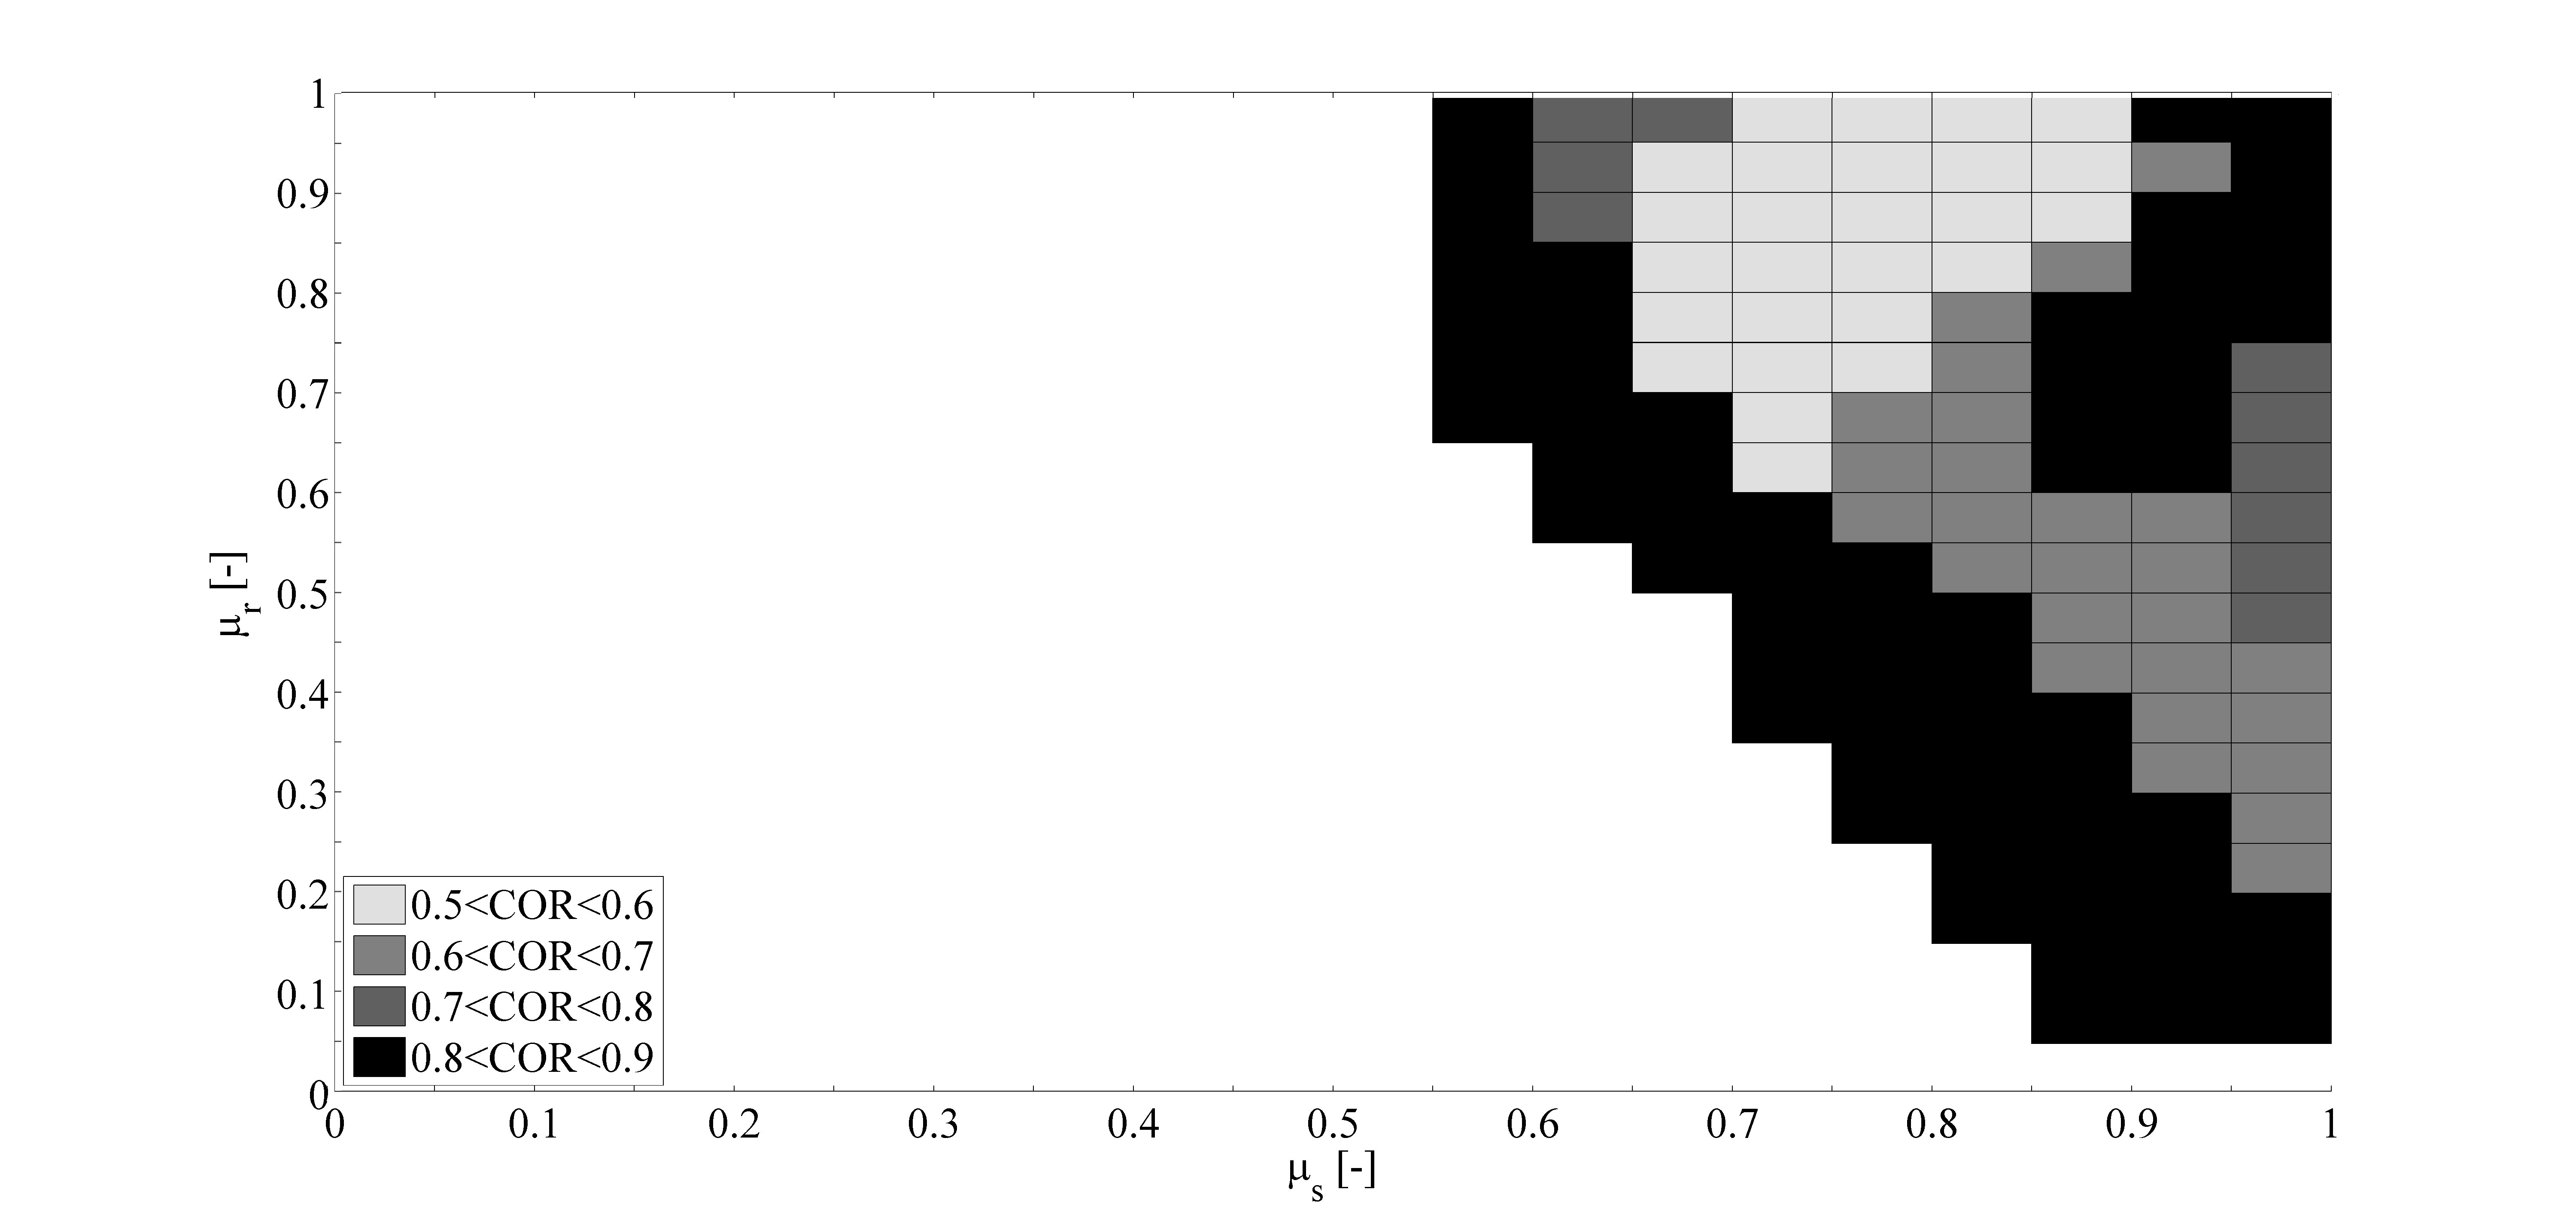
\includegraphics[width=\textwidth]{images/original/25cloudpirker1schulze10070}
        \caption{Cloud plot, $SCT$, $\sigma_n=10070 ~[Pa]$, $P=1.0$}
        \label{fig:25cloudpirker1schulze10070}
    \end{subfigure}\\
    \begin{subfigure}[b]{2cm}
        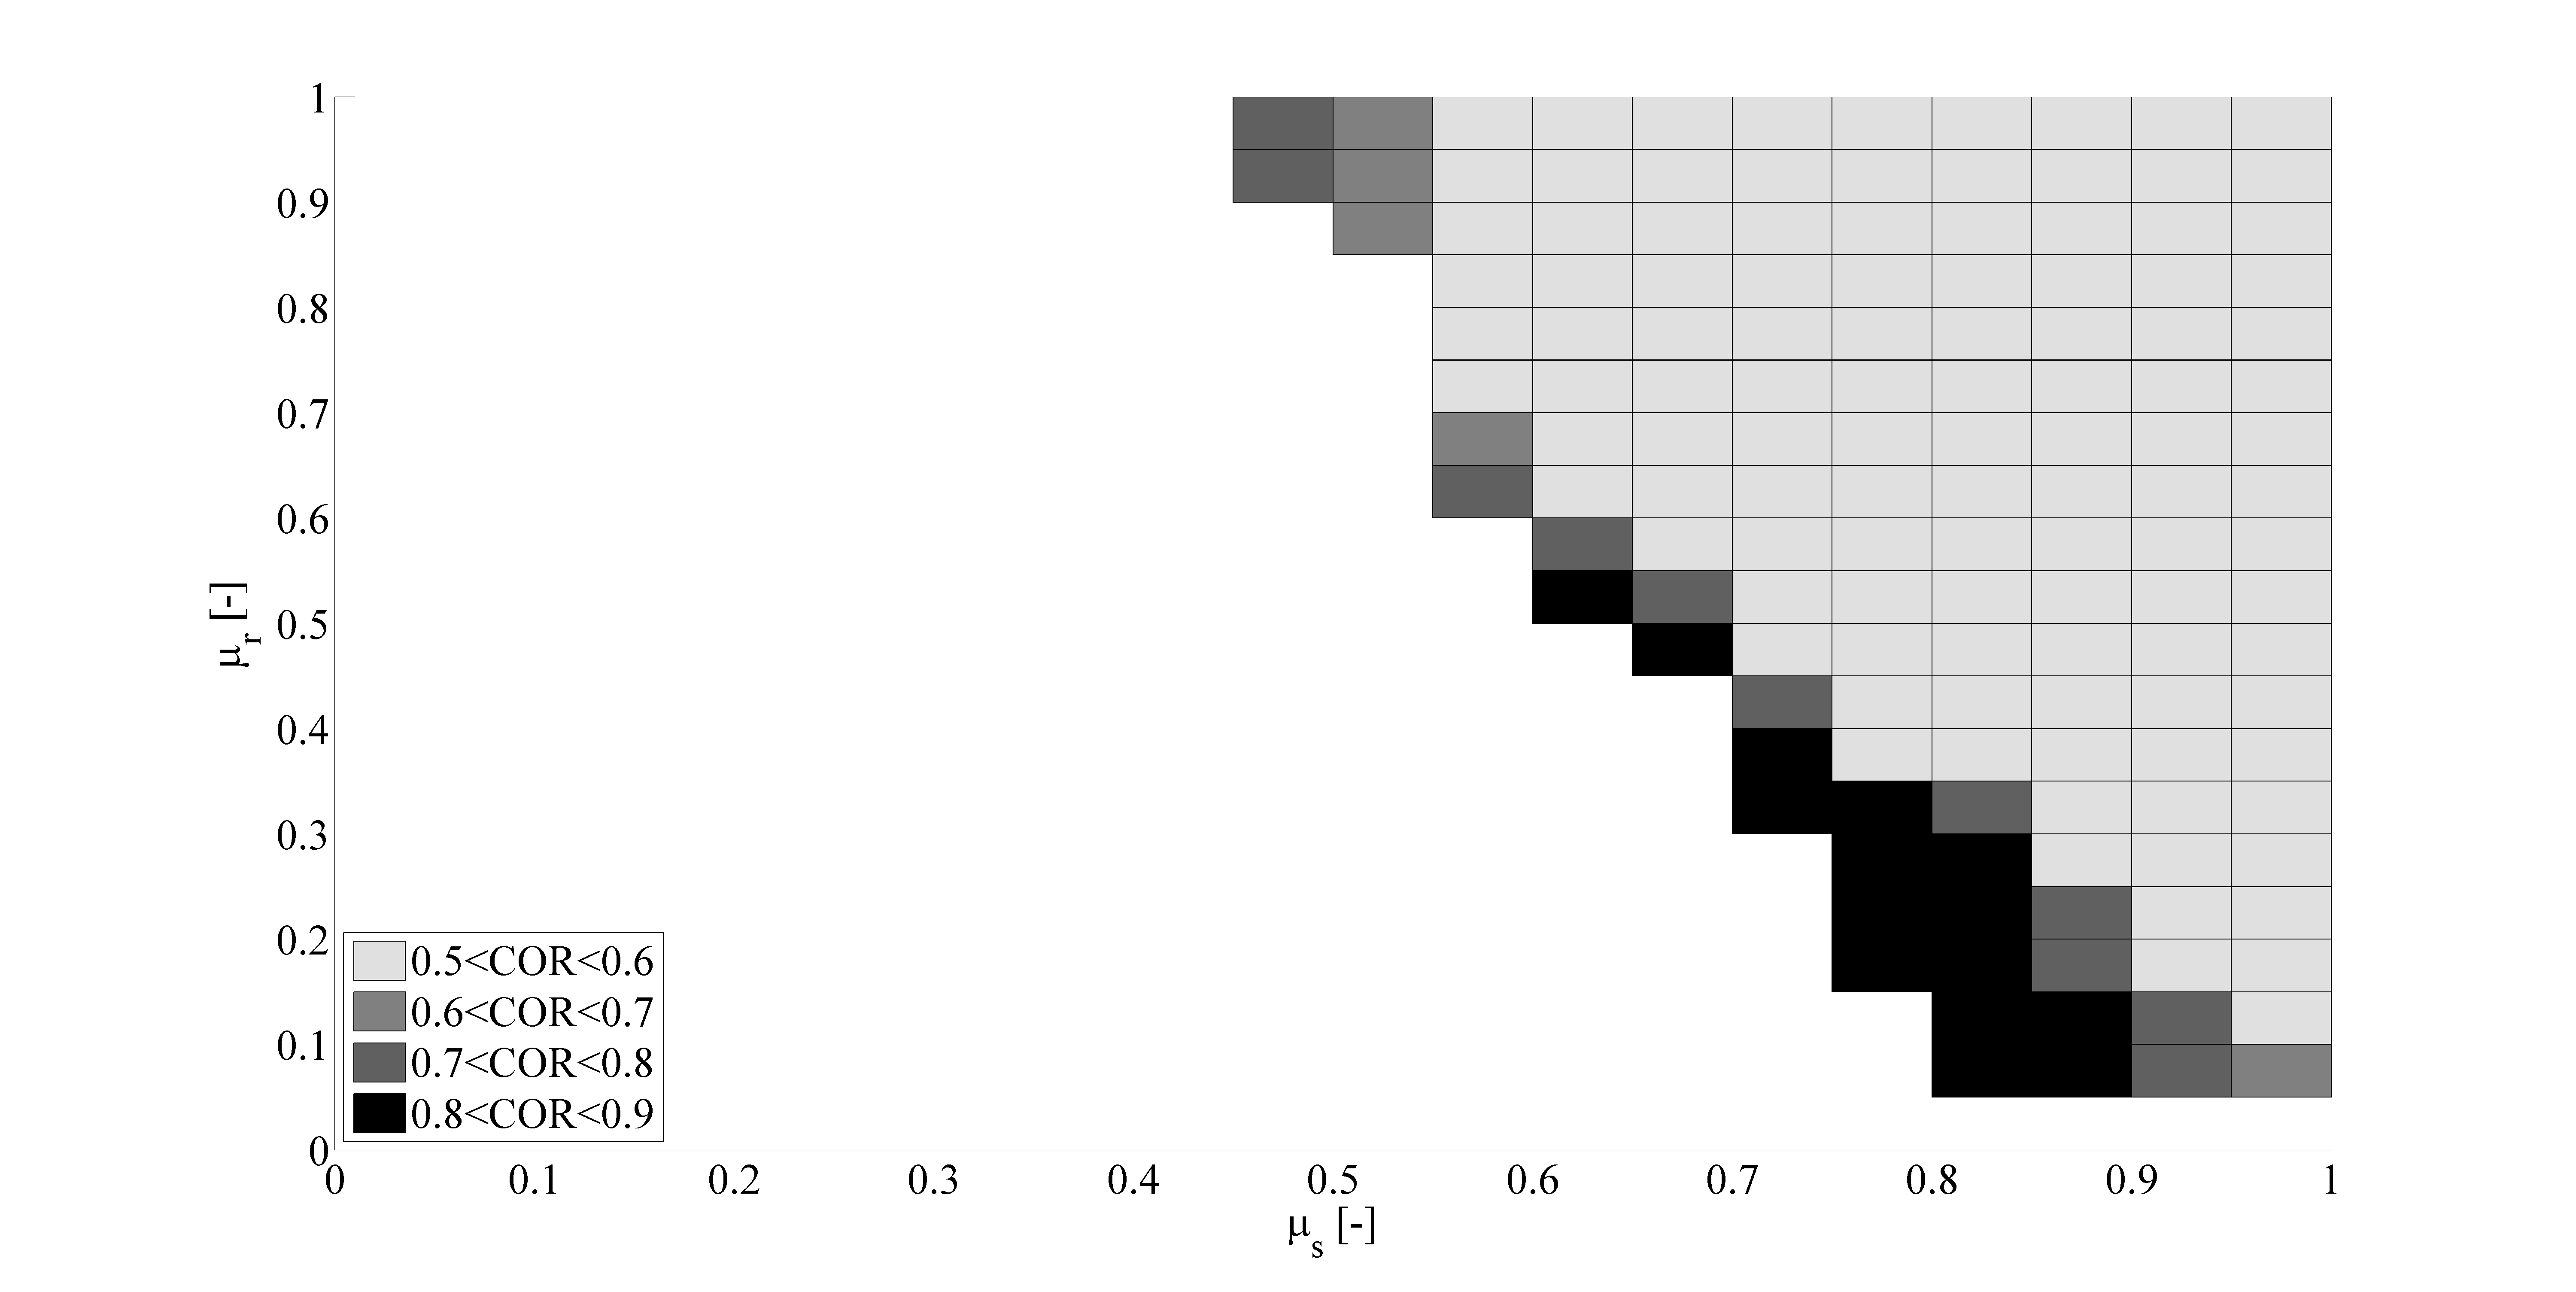
\includegraphics[width=\textwidth]{images/original/27cloudpirker08schulze10070}
        \caption{Cloud plot, $SCT$, $\sigma_n=10070 ~[Pa]$, $P=0.8$}
        \label{fig:27cloudpirker08schulze10070} 
    \end{subfigure}\\
    \begin{subfigure}[b]{2cm}
        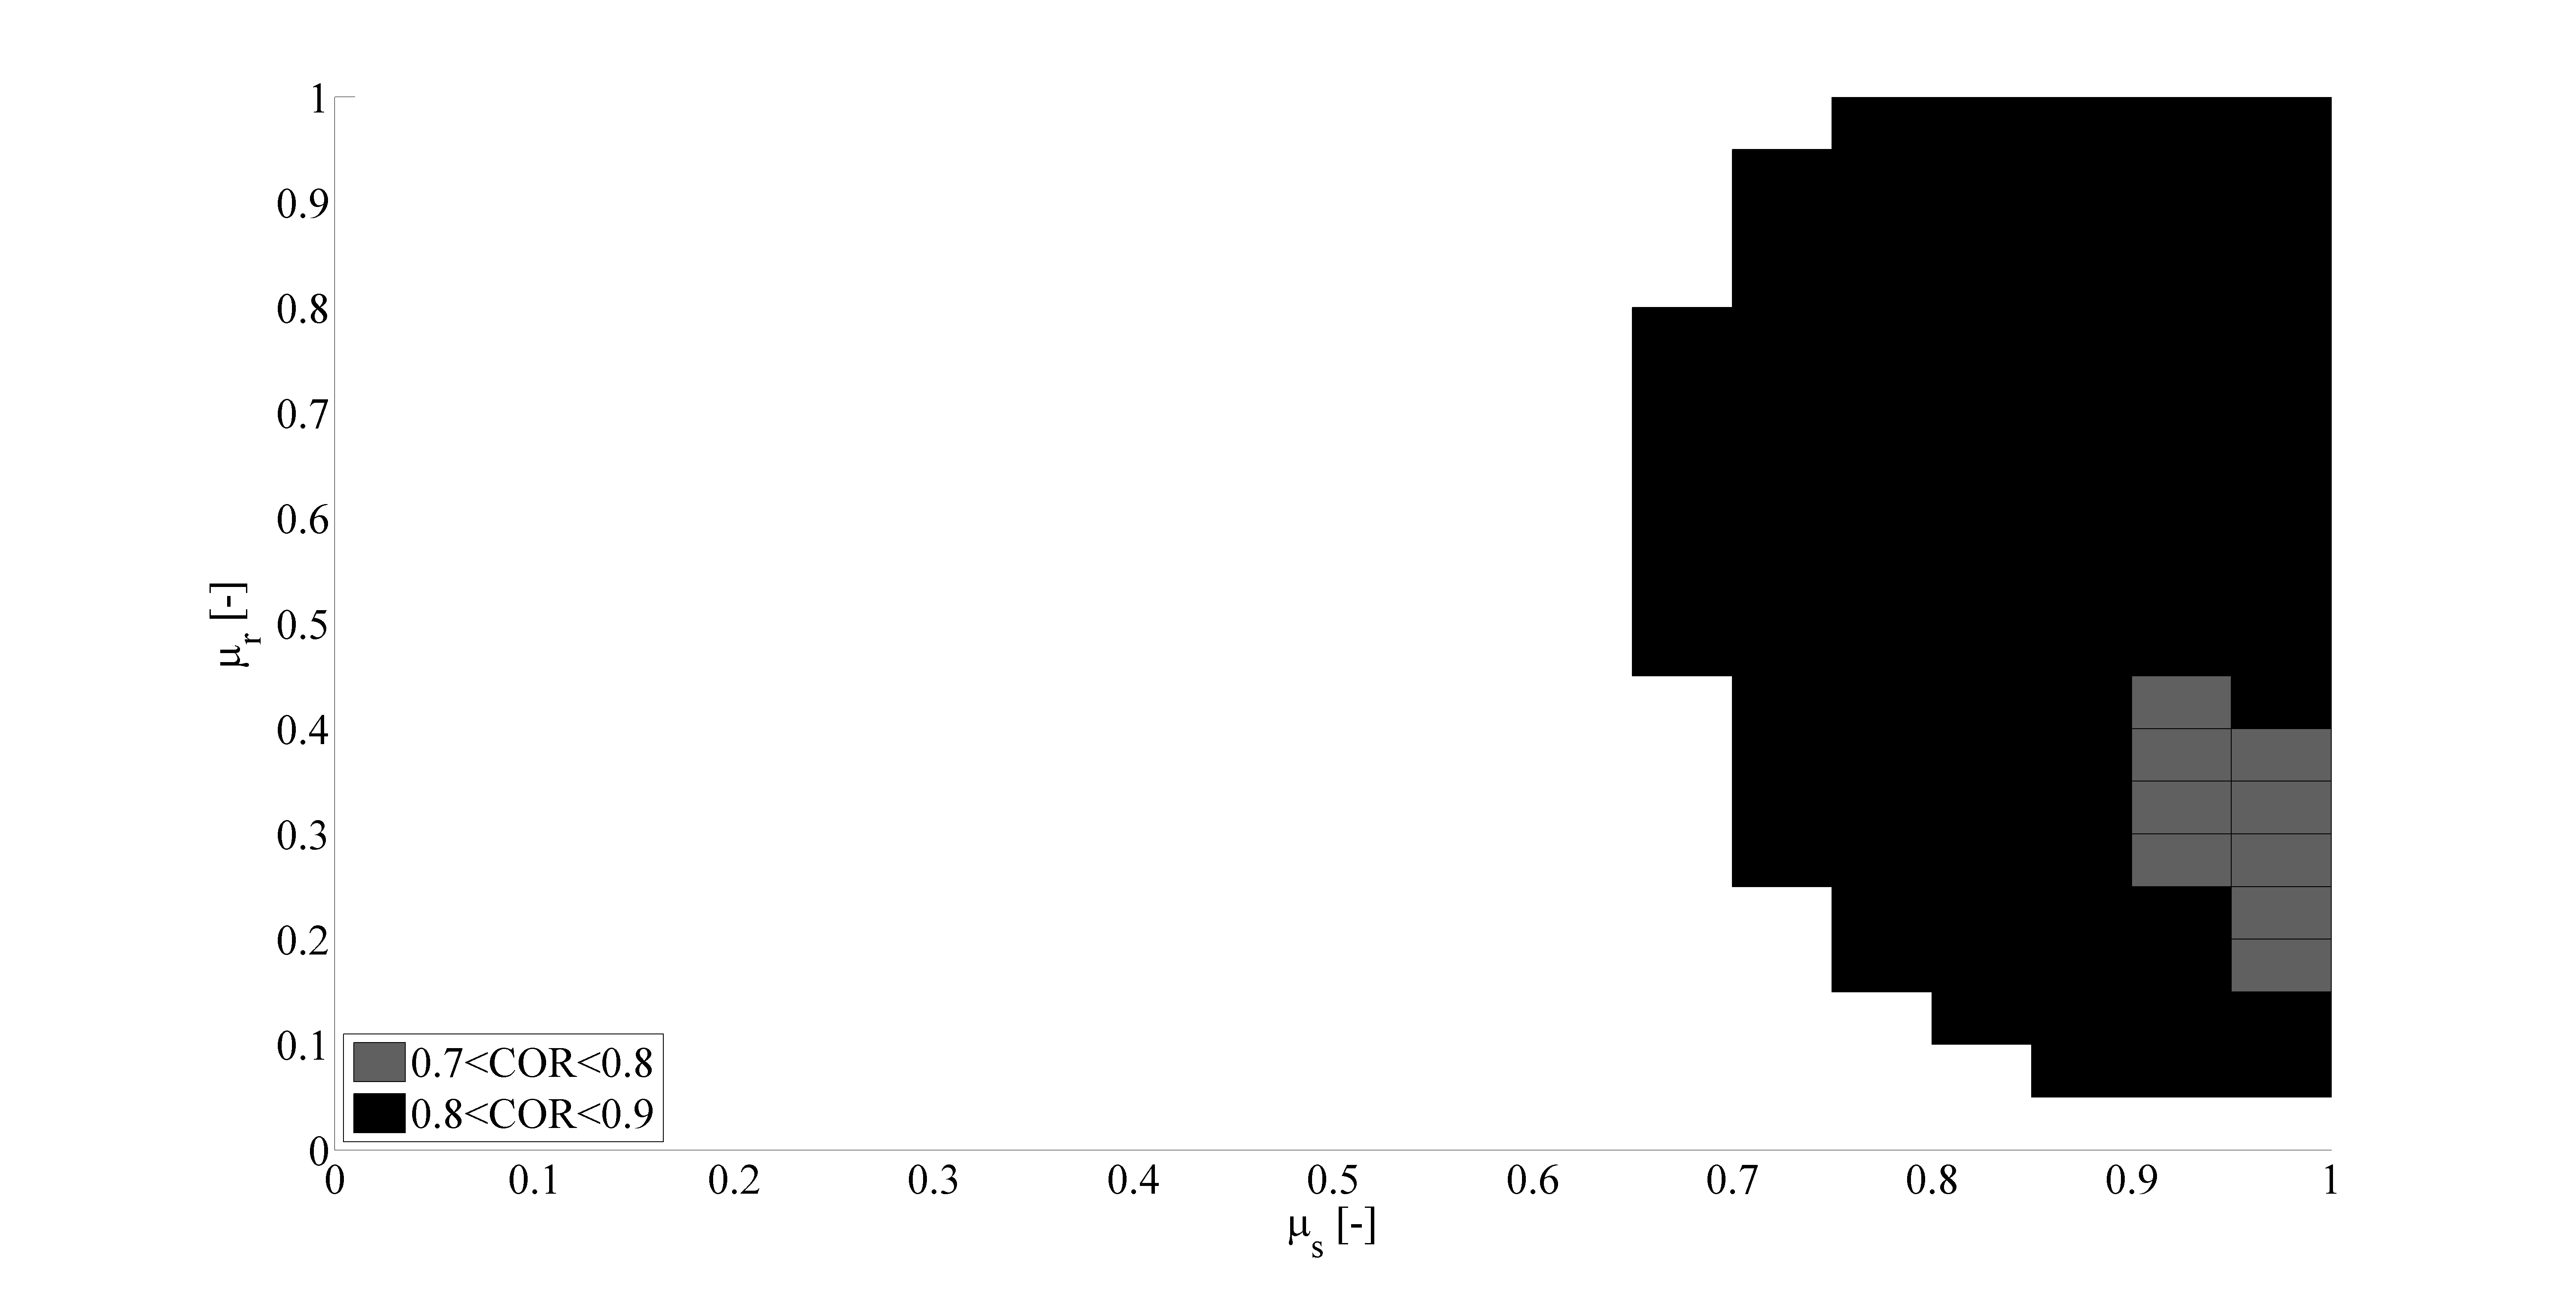
\includegraphics[width=\textwidth]{images/original/30cloudpirker12schulze10070}
        \caption{Cloud plot, $SCT$, $\sigma_n=10070 ~[Pa]$, $P=1.2$}
        \label{fig:30cloudpirker12schulze10070} 
    \end{subfigure}
    \caption[Density plot comparison of SCT results]{Density plot comparison of
    $SCT$ results. We represent the tabbed combinations for one load condition
    of the shear cell. 
    Density plot of the particles' coefficient of restitution (COR) in dependence
	of coefficient of sliding friction and coefficient of rolling friction; in the
	white area no valid sets of simulation parameter can be found.
	In each cell the valid sets are grouped accordingly to the 4 different COR
	ranges.
	Each cell is colored accordingly to the group with the most members. 
    Here, the values plotted are selected between the numerical
    values from the $NN$ with initially the original experimental results for the shear cell tester $P=1.0$ (Fig.
    \ref{fig:25cloudpirker1schulze10070}). 
        Later, they have been chosen with  
    the virtual decreased results $P=0.8$
    (\ref{fig:27cloudpirker08schulze10070}).
    The last image (Fig. \ref{fig:30cloudpirker12schulze10070}) represents
    instead the selection with the the virtual increased results $P=1.2$.    }
    \label{fig:29schulzeradarandcloud}
\end{figure}